\documentclass[aspectratio=43]{beamer}

\usetheme{simple}
\setbeamercovered{invisible}

\usepackage{qrcode}
\usepackage{lmodern}
\usepackage[scale=2]{ccicons}
\usepackage{multicol}
\usepackage{tikz}
\usepackage{graphicx}
\usepackage{subcaption}

\usepackage[utf8]{inputenc}
\usepackage[spanish]{babel}
\selectlanguage{spanish}
\usepackage{listings}
\usepackage{xcolor}

\definecolor{codegreen}{rgb}{0,0.6,0}
\definecolor{codegray}{rgb}{0.5,0.5,0.5}
\definecolor{codepurple}{rgb}{0.58,0,0.82}
\definecolor{backcolour}{rgb}{0.95,0.95,0.92}
\lstdefinestyle{mystyle}{
    backgroundcolor=\color{backcolour},
    commentstyle=\color{codegreen},
    keywordstyle=\color{magenta},
    numberstyle=\tiny\color{codegray},
    stringstyle=\color{codepurple},
    basicstyle=\ttfamily\footnotesize,
    breakatwhitespace=false,         
    breaklines=true,                 
    captionpos=b,                    
    keepspaces=true,                 
    numbers=left,                    
    numbersep=5pt,                  
    showspaces=false,                
    showstringspaces=false,
    showtabs=false,                  
    tabsize=2
}

\lstset{style=mystyle}
\def\edicion{}
\def\fecha{Octubre 2023}

\title{\textit{Linux404}}
\subtitle{Instalar Linux}
\author{José Antonio Verde Jiménez}
\date{Octubre 2023}
\github{joseaverde}

\institute{\edicion \ Talleres del GUL}
\date{\fecha}

\titlegraphic{img/logo1.png}
\begin{document}

    {
        \setbeamertemplate{footline}{}
        \frame{\titlepage}
    }
    \addtocounter{framenumber}{-1}
    \begin{frame}{Índice}
        \begin{multicols}{2}
            \tableofcontents

        \end{multicols}
    \end{frame}

    %=========================================================================%
    %==== Linux ==============================================================%
    %=========================================================================%
    \section{Linux}

    %== ¿Qué es Linux? ==%
    \subsection{¿Qué es Linux?}
    \begin{frame}
        \begin{multicols}{2}
            Linux es un sistema operativo:
            \begin{itemize}
                \item Libre
                \item De Código Abierto
                \item \textbf{Gratis} (en su gran mayoría)
            \end{itemize}

            \newpage

            \begin{figure}[b]
                
\includegraphics[width=0.4\textwidth]{img/tux.png}
                \caption*{\textit{Tux}, mascota de Linux}
            \end{figure}
        \end{multicols}
    \end{frame}

    %== Distros ==%
    \subsection{Distros}
    % En realidad os he mentido, hay muchos Linux.
    % ¿Cuál uso?
    \begin{frame}{\secname}{\subsecname}
        \textbf{Más populares}
        \begin{figure}[b]
            \centering
            \begin{subfigure}{.3\textwidth}
                \centering
                
\includegraphics[width=0.35\textwidth]{img/mx.png}
            \end{subfigure}
            \begin{subfigure}{.3\textwidth}
                \centering
                
\includegraphics[width=0.35\textwidth]{img/mint.png}
            \end{subfigure}
            \begin{subfigure}{.3\textwidth}
                \centering
                
\includegraphics[width=0.35\textwidth]{img/endeavour.png}
            \end{subfigure}
            \centering
            \begin{subfigure}{.3\textwidth}
                \centering
                
\includegraphics[width=0.35\textwidth]{img/debian.png}
            \end{subfigure}
            \begin{subfigure}{.3\textwidth}
                \centering
                
\includegraphics[width=0.35\textwidth]{img/ubuntu.png}
            \end{subfigure}
            \begin{subfigure}{.3\textwidth}
                \centering
                
\includegraphics[width=0.35\textwidth]{img/manjaro.png}
            \end{subfigure}
            \centering
            \begin{subfigure}{.3\textwidth}
                \centering
                
\includegraphics[width=0.35\textwidth]{img/popos.png}
            \end{subfigure}
            \begin{subfigure}{.3\textwidth}
                \centering
                
\includegraphics[width=0.35\textwidth]{img/fedora.png}
            \end{subfigure}
            \begin{subfigure}{.3\textwidth}
                \centering
                
\includegraphics[width=0.35\textwidth]{img/opensuse.png}
            \end{subfigure}
        \end{figure}
        \begin{multicols}{3}
            \pause
            \centering \textbf{Ciberseguridad}
            \begin{figure}
                
\includegraphics[width=0.1\textwidth]{img/kali.png}
                
\includegraphics[width=0.1\textwidth]{img/parrot.png}
            \end{figure}
            \newpage
            \pause
            \centering \textbf{Avanzadas}
            \begin{figure}
                
\includegraphics[width=0.07\textwidth]{img/arch.png}
                
\includegraphics[width=0.07\textwidth]{img/gentoo.png}
            \end{figure}
            \begin{figure}
                
\includegraphics[width=0.07\textwidth]{img/lfs.png}
                
\includegraphics[width=0.07\textwidth]{img/nixos.png}
            \end{figure}
            \newpage
            \pause
            \centering \textbf{\textit{Otras}}
            \begin{figure}
                
\includegraphics[width=0.07\textwidth]{img/tinycore.png}
                
\includegraphics[width=0.07\textwidth]{img/redstaros.png}
            \end{figure}
            \begin{figure}
                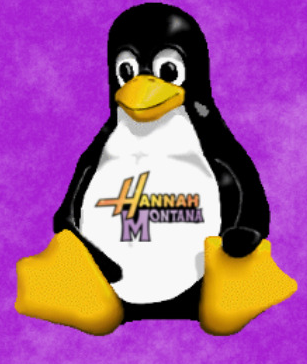
\includegraphics[width=0.05\textwidth]{img/hannah.png}
            \end{figure}
        \end{multicols}
    \end{frame}

    \begin{frame}{\secname}{\subsecname}
        \centering
        \begin{figure}
            
\includegraphics[width=0.8\textwidth]{img/distrochooser.png}
        \end{figure}
        \centering \url{https://distrochooser.de/es}
    \end{frame}

    %== ¿Cómo se ve Linux? ==%
    \subsection{¿Cómo se ve Linux?}
    \begin{frame}{\secname}{\subsecname}
        \begin{figure}
            \centering
            \begin{subfigure}{.4\textwidth}
                \centering
                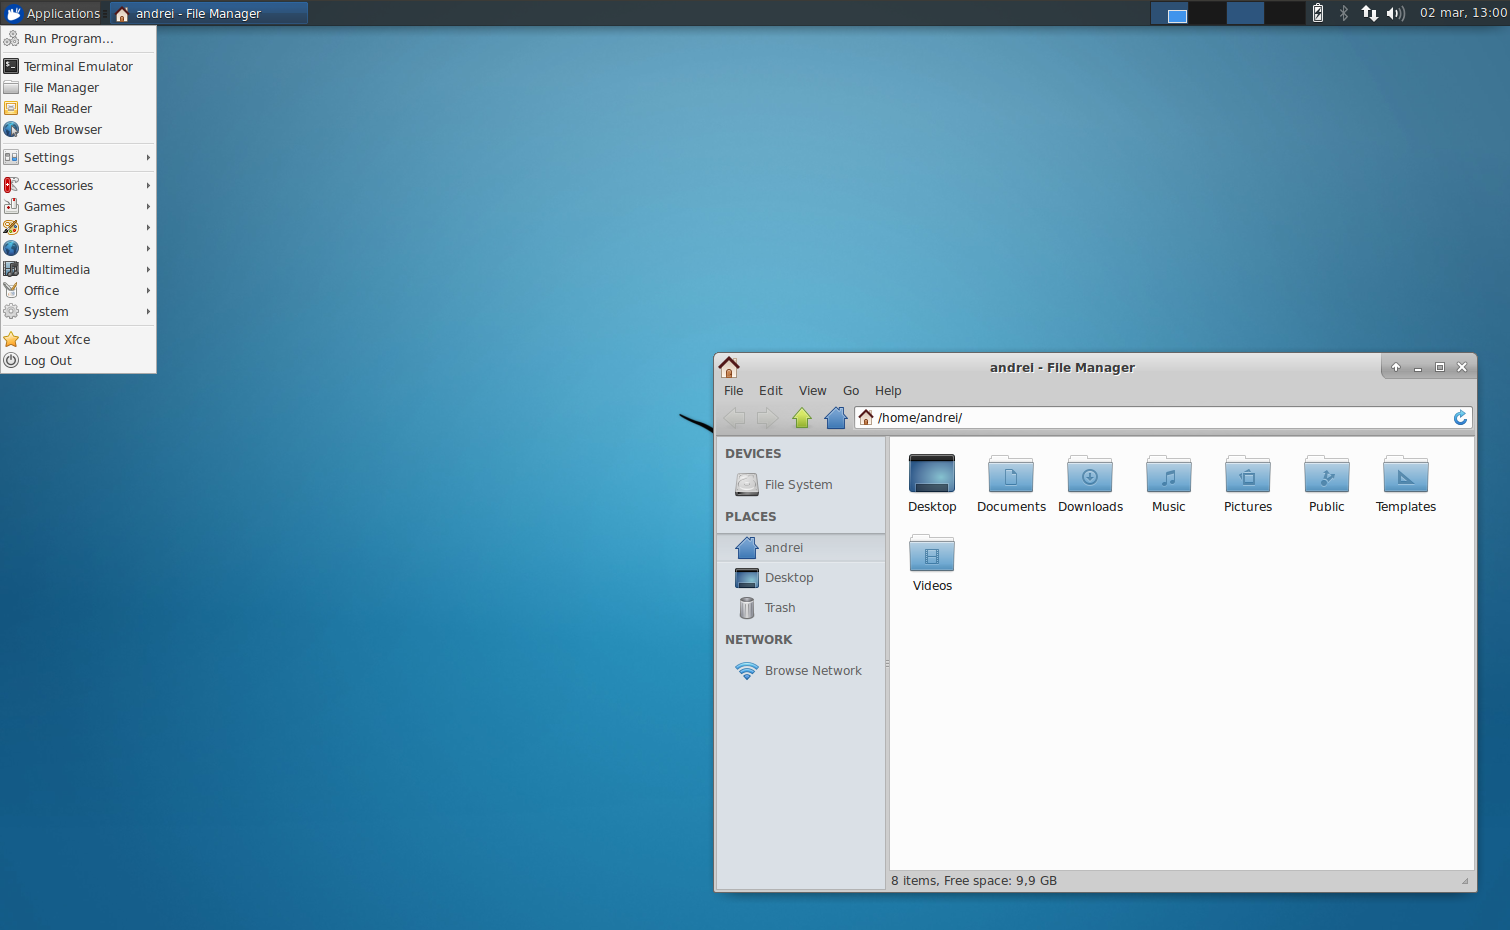
\includegraphics[width=\textwidth]{img/xfce4.png}
                \caption*{Xfce4}
            \end{subfigure}
            \begin{subfigure}{.4\textwidth}
                \centering
                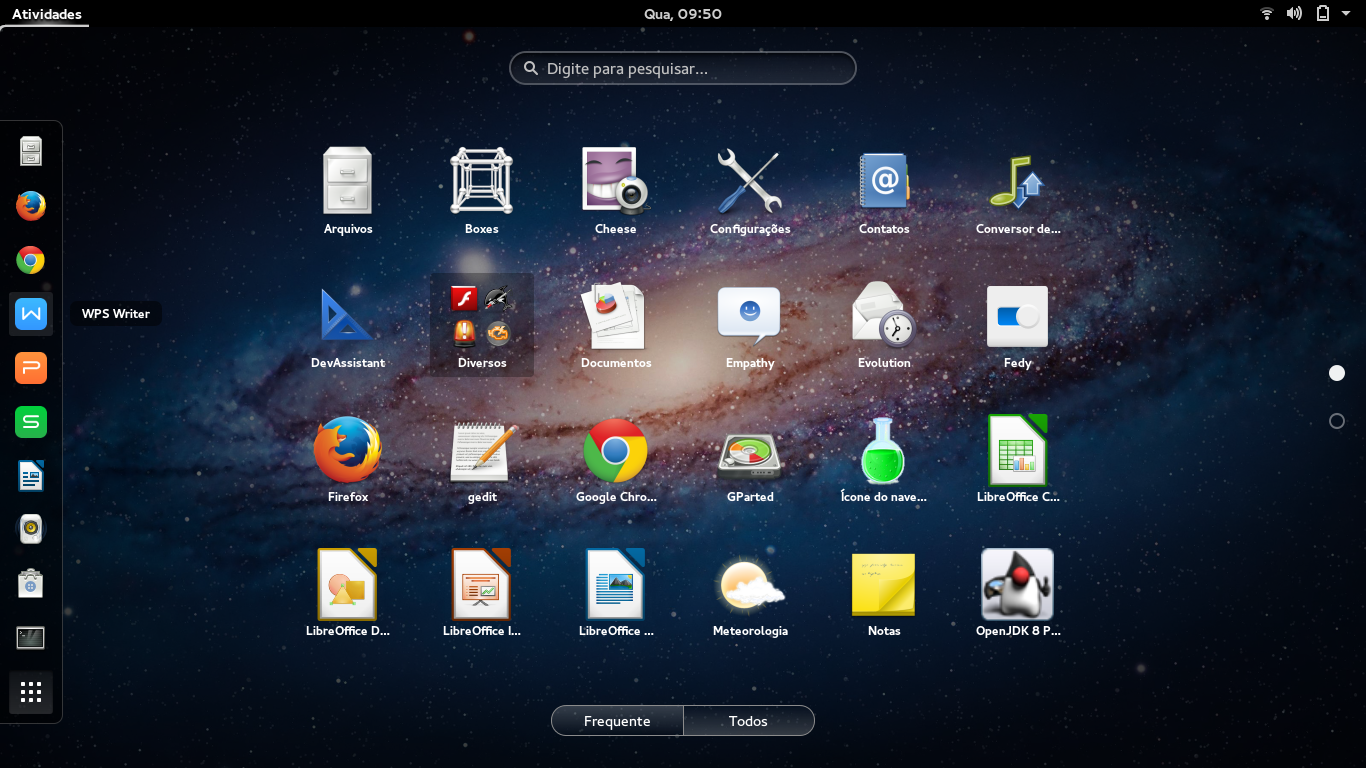
\includegraphics[width=\textwidth]{img/gnome.png}
                \caption*{GNOME}
            \end{subfigure}
        \end{figure}
        \begin{figure}
            \centering
            \begin{subfigure}{.4\textwidth}
                \centering
                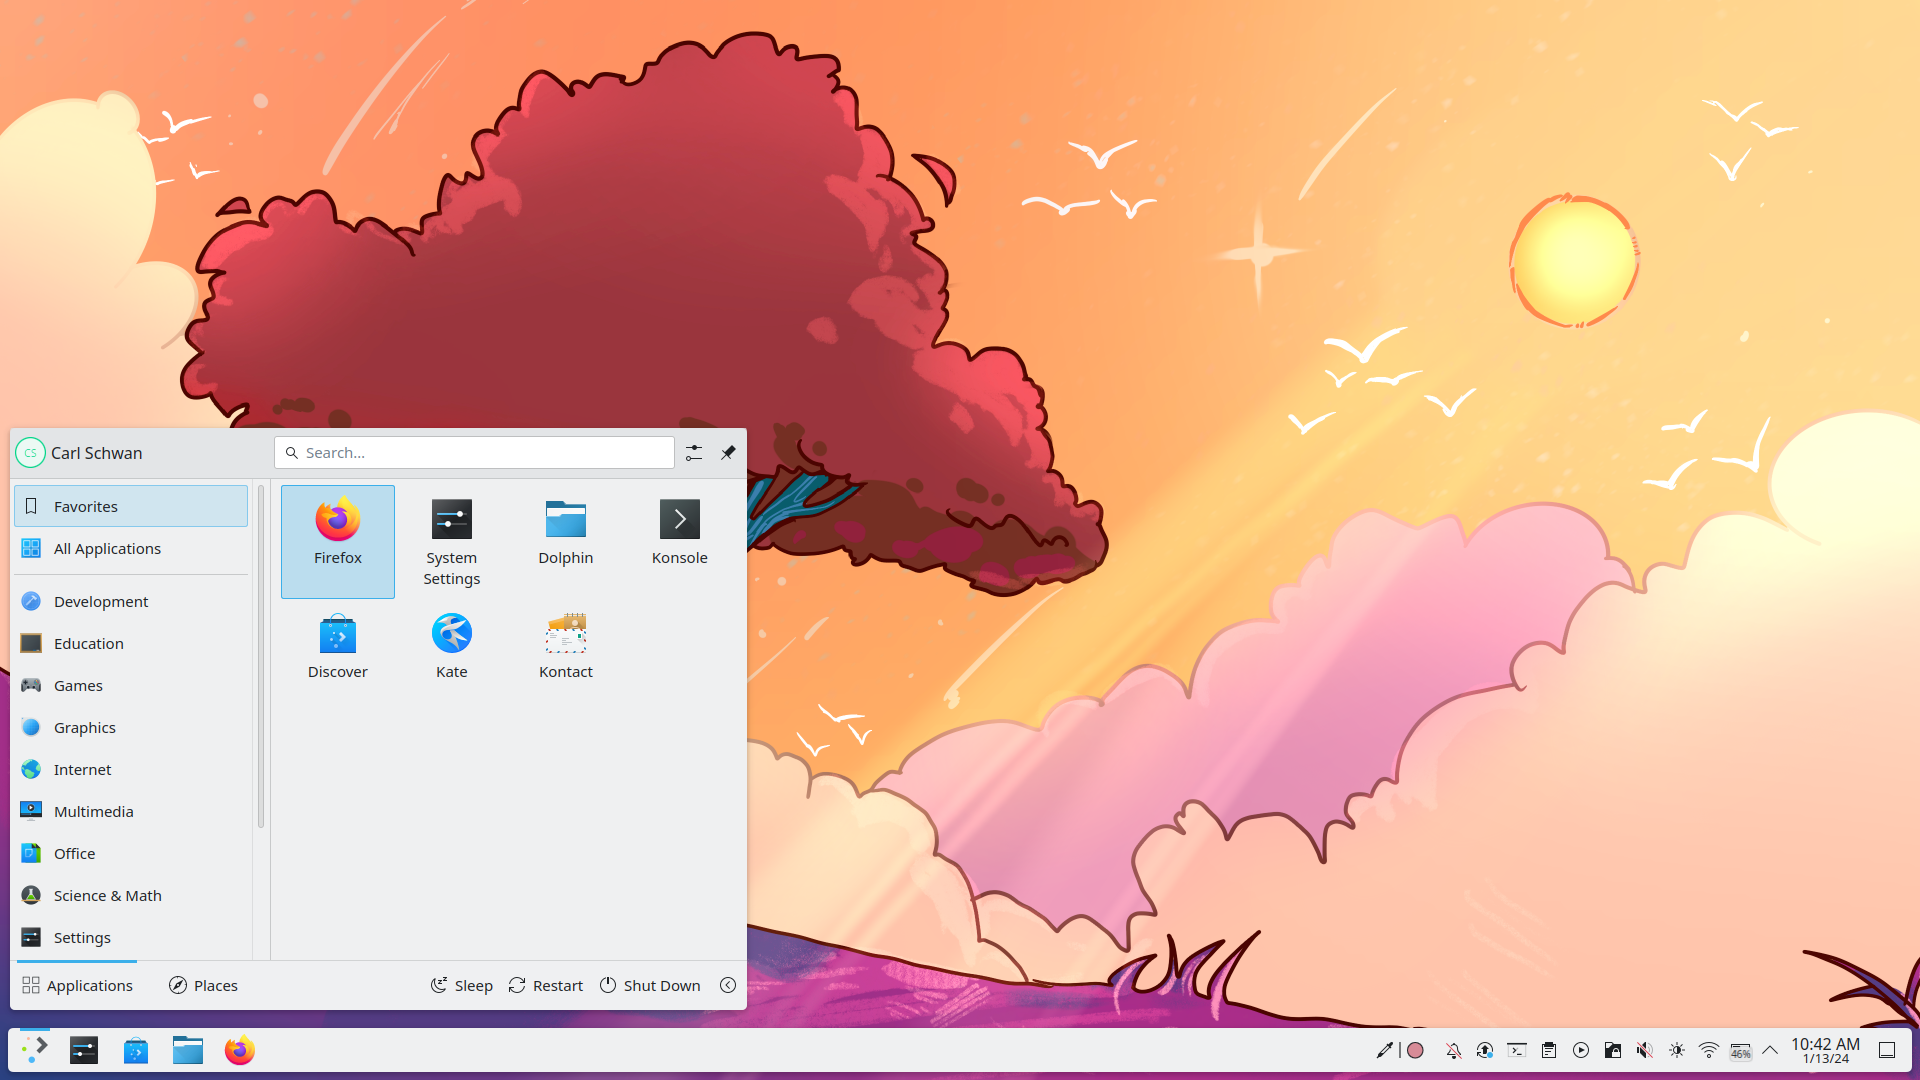
\includegraphics[width=\textwidth]{img/kde.png}
                \caption*{KDE}
            \end{subfigure}
            \begin{subfigure}{.4\textwidth}
                \centering
                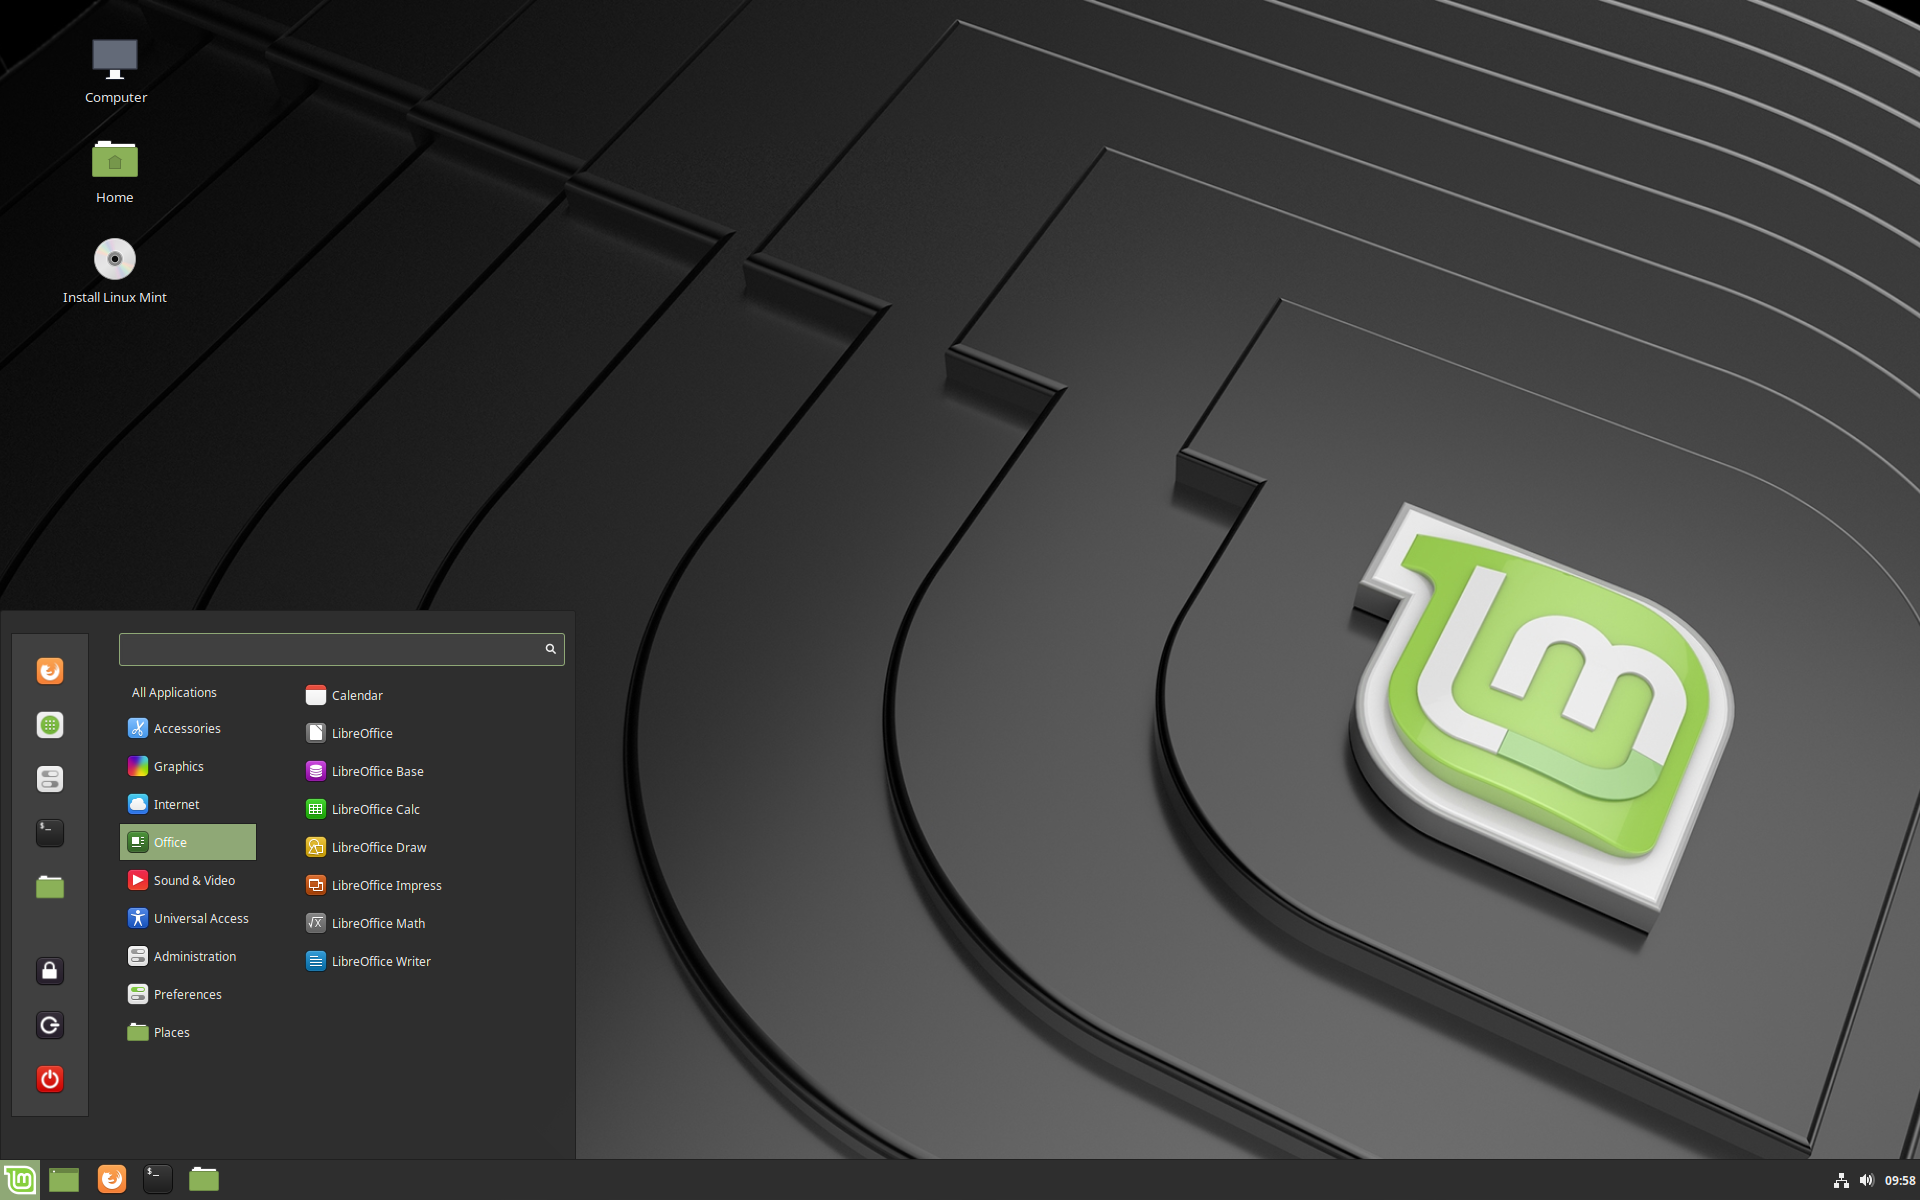
\includegraphics[width=\textwidth]{img/cinnamon.png}
                \caption*{Cinnamon}
            \end{subfigure}
        \end{figure}
    \end{frame}

    %== ¿Por qué Linux? ==%
    \subsection{¿Por qué Linux?}
    \begin{frame}{\secname}{\subsecname}
        \begin{itemize}
            \item Es fácil de utilizar.
            % Los que nunca han utilizado Linux dicen que es difícil
            \item Seguro
            % Ya ves lo usa mucha gente
            \item Código abierto
            \item Rápido
            \item Revive ordenadores antiguos
            \item Todo lo que necesites está en la tienda de aplicaciones
            \item Se usa mucho más de lo que parece:
            \begin{itemize}
                \item El $7.23\%$ de los ordenadores personales.
                \item El $38.42\%$ de los sistemas embebidos.
                \item El $77.4\%$ de los servidores
                \item El $70.8\%$ de los dispositivos móviles
                \item El $100\%$ de las supercomputadoras.
            \end{itemize}
            \item Libre de publicidad.
            \item Respeta tu privacidad.
        \end{itemize}
    \end{frame}

    %== Falsos Mitos ==%
    \subsection{Falsos mitos}
    \begin{frame}[fragile]{\subsecname}{\secname}
        \begin{itemize}
            \item \textit{«He oído que necesitas la terminal para todo»}
            \pause
            \begin{itemize}
                \item Tienes una aplicación gráfica para la tienda de aplicaciones
                \item Puedes personalizar el sistema con un menú gráfico
                \item Hay aplicaciones para configurar los \textit{drivers}.
            \end{itemize}
            Es una comodidad para el usuario intermedio-avanzado.
            \item «Los programas de Windows no funcionan en Linux y necesito\ldots»
            \pause
            \begin{itemize}
                \item Tienes \verb!wine!.
                \item Hay una base de datos
                    \href{(WineHQ)}{https://appdb.winehq.org/} con información
                    de cómo configurar muchas aplicaciones.
            \end{itemize}
            \item «En Linux no se puede jugar a videojuegos»
            \pause
            \begin{itemize}
                \item Steam con \textit{Proton}
                \item \textit{PlayOnLinux}
                \item \textit{Lutris}
            \end{itemize}
        \end{itemize}
    \end{frame}

    %=========================================================================%
    %==== Preliminares =======================================================%
    %=========================================================================%
    \section{Preliminares}

    \subsection{Físico v.s. Máquina Virtual}
    \begin{frame}{\secname}{\subsecname}
        \begin{multicols}{2}
            \textbf{Físico}
            \begin{enumerate}
                \item \textbf{Pros}
                \begin{enumerate}
                    \item Rápido
                    \item Usa tarjeta gráfica
                    \item Acceso a periféricos
                    \item Más cómodo
                    \item Aprovecha el \textit{Hardware}
                \end{enumerate}
                \item \textbf{Contras}
                \begin{enumerate}
                    \item Tamaño fijo
                    \item Reiniciar para cambiar
                \end{enumerate}
            \end{enumerate}
            \newpage
            \textbf{Máquina virtual}
            \begin{itemize}
                \item \textbf{Pros}
                \begin{itemize}
                    \item Tamaño variable
                    \item Tantas imágenes abiertas como quieras
                \end{itemize}
                \item \textbf{Contras}
                \begin{itemize}
                    \item Más lento
                    \item No aprovecha el \textit{Hardware}
                \end{itemize}
            \end{itemize}
        \end{multicols}
        \begin{multicols}{2}
            \begin{figure}
                \centering
                
\includegraphics[width=0.3\textwidth]{img/gparted.png}
            \end{figure}
            \begin{figure}
                \centering
                
\includegraphics[width=0.2\textwidth]{img/virtualbox.png}
            \end{figure}
        \end{multicols}
    \end{frame}

    \subsection{Para los que se lo quieren instalar en físico}
    \begin{frame}[fragile]{\subsecname}{\secname}
        \url{https://github.com/guluc3m/linux404} (dualboot-install.md)
        \begin{enumerate}
            \pause
            \item Desfragmentar el disco
            \begin{enumerate}
                \item Buscar \textbf{Defrag} en la barra de búsqueda
                \item \textbf{Desframentar y optimizar unidades}
                \item Seleccionar disco (normalmente \verb!C:\!).
                \item \textbf{Optimizar}
            \end{enumerate}
            \pause
            \item (Windows 11) Desactivar \textit{BitLocker}
            \pause
            \begin{enumerate}
                \item Buscar \textbf{BitLocker}, si no aparece, genial.
                \item Copia de seguridad de la clave
                \item Desactiva \textit{BitLocker}
            \end{enumerate}
            \pause
            \item Desactivar inicio rápido
            \begin{enumerate}
                \item Buscar \textbf{Opciones de Energía}
                \item \textbf{Comportamiento de los botones de inicio/apagado}
                \item Desactiva inicio rápido
                \item \textbf{Guardar Cambios}
                \item Si no aparece, ejecutar \verb!powercfg.exe /h on! y
                cuando termines \verb!powercfg.exe /h off! en una CMD.
            \end{enumerate}
        \end{enumerate}
    \end{frame}
    % Si alguien ha traído un Pen Drive vacío, y no hay suficientes podemos ir
    %   ayudando.

    \subsection{Para los que se lo quieren instalar en una máquina virtual}
    \begin{frame}{\secname}{\subsecname}
        \url{https://github.com/guluc3m/linux404} (vm-install.md)
        \begin{enumerate}
            \item Descargar VirtualBox
            \item Descargar la distro que quieras
            \item Instalar VirtualBox
            \item Sigue las instrucciones. Dale suficiente almacenamiento
                (por ejemplo 32GiB), unos cuantos procesadores y bastante
                memoria RAM.
        \end{enumerate}
    \end{frame}
    % Si no se ha descargado para entonces copiarla de una Pen Drive.

    \subsection{Particiones}
    \begin{frame}[fragile]{\secname}{\subsecname}
        \begin{figure}
            \centering
            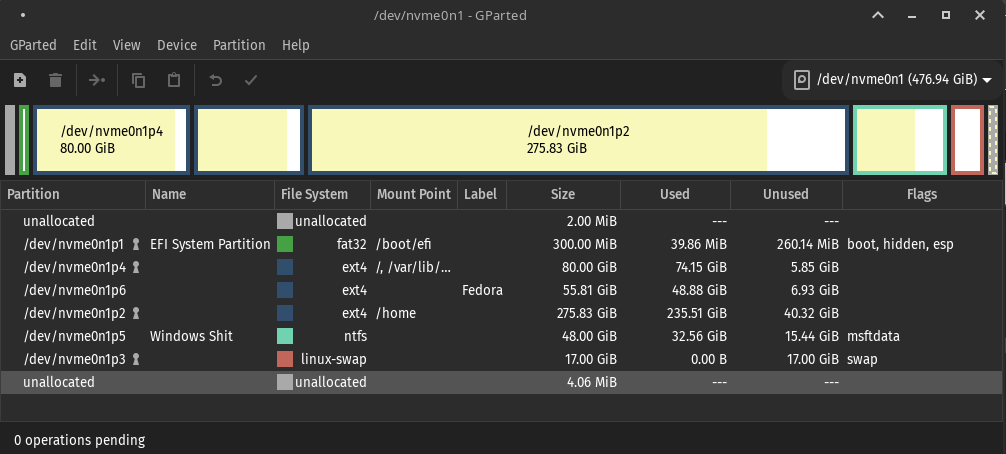
\includegraphics[width=0.9\textwidth]{img/partitions.png}
        \end{figure}
        \begin{itemize}
            \item \verb!/! (\textit{root}, S.O.)
            \item \verb!/home! (Archivos personales)
            \item \verb!EFI! (Gestor de Arranque)
            \item \verb!swap! (Área de intercambio)
        \end{itemize}
    \end{frame}
    % Explicar que estamos dividiendo el disco en distintas partes lógicas
    % Explicar qué pueden hacer /home /boot /efi / ...
    % Mandar a que una vez se haya terminado de desfragmentar, que reduzcan el
    %   espacio que ocupa Windows. Es preferible que Windows se corte el brazo
    %   a sí mismo; a que se despierte sin un brazo.
    % Hay una opción muy bonita que se llama instalar al lado de Windows que se
    %   decide por ti.

    \subsection{BIOS}
    \begin{frame}[fragile]{\secname}{\subsecname}
        \begin{itemize}
            \item Apaga el ordenador
            \item Enciende utilizando el botón para entrar en la BIOS
            (\verb!ESC!, \verb!F11!, \verb!F12!, \verb!DEL!)
            \item Asegúrate que \textit{Intel(R) Rapid Start Technology} está
            \textbf{desactivado}
            \item Si estás instalando una distro \textbf{distinta a Ubuntu},
            \textbf{desactivar} \textit{«Secure Boot»}
            \item Arranca desde el USB.
        \end{itemize}
    \end{frame}
    % Pedir que vayan buscando para su modelo de ordenador qué tecla utilizar
    %   para entrar en BIOS.
    % Si no están instalando Ubuntu, pedir que desactiven el Secure Boot

    % \subsection{Arranque}
    % Una vez lo tengan todos, arrancar desde Linux
    % No se va a instalar nada todavía.

    %=========================================================================%
    %==== Instalación ========================================================%
    %=========================================================================%
    \section{Instalación}
    \subsection{Configuración}
    \begin{frame}{\secname}{\subsecname}
        \begin{itemize}
            \item Seleccionar \textit{Install Linux}
            \item Para la \textit{eduroam} usad la siguiente configuración:
            \begin{itemize}
                \item \textbf{\textit{Security}}: \textit{WPA/WPA2 Enterprise}
                \item \textbf{\textit{Authentication}}: \textit{Tunnelled TLS}
                \item Selecciona \textit{No CA certificate is required}
                \item \textbf{\textit{Inner authentication}}: \textit{MSCHAPv2 (no EAP)}
                \item \textbf{\textit{Username}}: El N.I.A.
                \item \textbf{\textit{Password}}: La contraseña de aula global.
            \end{itemize}
            \item Si lo pregunta, activad códecs multimedia
            \item Parad cuando lleguéis a la parte de particionado.
        \end{itemize}
    \end{frame}
    % WiFi de la uni - En una máquina virtual no es necesario
    % Instalar códecs de vídeo
    % Que se paren cuando lleguen a las particiones.

    \subsection{Particionado}
    \begin{frame}[plain]
        \begin{tikzpicture}[overlay, remember picture]
            \node[anchor=center] at (current page.center) {
                \begin{beamercolorbox}[center]{title}
                    \huge Particionado
                \end{beamercolorbox}};
        \end{tikzpicture}
    \end{frame}
    % Vamos a pasar por las mesas para hacer el siguiente paso.
    % En una máquina virtual que usen el disco entero
    % Continuar

    %=========================================================================%
    %==== Introducción =======================================================%
    %=========================================================================%
    \section{Introducción}
    \subsection{Gestores de Paquetes}
    \begin{frame}[fragile]{\secname}{\subsecname}
        \begin{multicols}{2}
            \textbf{APT} (Debian, Ubuntu, Mint\ldots)\\
            \begin{lstlisting}[language=bash]
$ sudo apt update
$ sudo apt upgrade
$ sudo apt install <paquete>
$ sudo apt remove <paquete>
$ sudo apt search <paquete>
$ man apt \end{lstlisting}
            \textbf{dnf} (Fedora, RedHat\ldots)\\
            \begin{lstlisting}[language=bash]
$ sudo dnf check-update
$ sudo dnf upgrade
$ sudo dnf install <paquete>
$ sudo dnf remove <paquete>
$ sudo dnf search <paquete>
$ man dnf \end{lstlisting}
            \newpage
            \textbf{pacman} (Arch, Manjaro\ldots)\\
            \begin{lstlisting}[language=bash]
$ sudo pacman -Sy
$ sudo pacman -Syu
$ sudo pacman -S <paquete>
$ sudo pacman -R <paquete>
$ sudo pacman -Ss <paquete>
$ man pacman \end{lstlisting}
            \textbf{Alternativas}
            \begin{itemize}
                \item \textbf{synaptic}: Debian, Ubuntu\ldots
                \item \textbf{nala}: Debian, Ubuntu\ldots
                \item \textbf{aptitude}: Debian, Ubuntu\ldots
                \item \textbf{Tienda de aplicaciones}
            \end{itemize}
        \end{multicols}
    \end{frame}
    \subsection{Juego: Adivina qué hace el comando}
    \begin{frame}[fragile]{\secname}{\subsecname}
        \begin{lstlisting}[language=bash]
sudo rm -fr /*\end{lstlisting}
        \begin{itemize}
            \item \textit{«¿Borrar el idioma francés del sistema?»}
            \pause\\
            \item \textbf{Borra el disco duro entero}
        \end{itemize}
        \begin{lstlisting}[language=bash]
:(){ :|:& };:\end{lstlisting}
        \begin{itemize}
            \item \textit{«¿No hace nada?}
            \pause\\
            \item \textbf{Es una bomba lógica}
        \end{itemize}
        \begin{lstlisting}[language=bash]
sudo dd if=/dev/random of=/dev/sda\end{lstlisting}
        \begin{itemize}
            \item \textit{«¿Genera un número aleatorio?}
            \pause\\
            \item \textbf{Te destruye el disco duro}
        \end{itemize}
        \pause
        \textbf{No ejecutes nada que no sepas que hace}
    \end{frame}
    % Nunca ejecutes algo que no sepas qué hace
    % Fuentes

    \subsection{Línea de Comandos}
    \begin{frame}[fragile]{\secname}{\subsecname}
        \begin{itemize}
            \item \verb!ls!: LiStar qué hay en el directorio actual.
            \item \verb!cd!: Cambiar de Directorio
            \item \verb!pwd!: \textit{Print Working Directory}
            \item \verb!rm!: ReMove (Borrar un archivo)
            \item \verb!cp!: CoPiar un archivo
            \item \verb!mv!: MoVer un archivo
            \item \verb!cat!: Imprimir qué hay dentro de un archivo
            \item \verb!nano!: Editar un archivo
            \item \verb|!!|: Ejecutar el comando anterior
            \item \verb|sudo|: \textit{Super User DO} (Ejecutar como súper usuario)
        \end{itemize}
        \pause
        \begin{itemize}
            \item \verb!.!: Directorio actual
            \item \verb!..!: Directorio superior
            \item \verb!/!: Directorio raíz
            \item \verb!~!: Directorio \verb!$HOME!
            \item \verb!-!: Directorio anterior
        \end{itemize}
    \end{frame}

    \subsection{Ejecutar programas de Windows}
    \begin{frame}{\secname}{\subsecname}
        \begin{figure}
            \centering
            \begin{subfigure}{.4\textwidth}
                \centering
                
\includegraphics[width=0.4\textwidth]{img/wine.png}
                \caption*{Wine}
            \end{subfigure}
            \pause
            \begin{subfigure}{.4\textwidth}
                \centering
                
\includegraphics[width=0.4\textwidth]{img/lutris.png}
                \caption*{Lutris (\url{https://lutris.net/})}
            \end{subfigure}
            \pause
        \end{figure}
        \begin{figure}
            \centering
            \begin{subfigure}{.4\textwidth}
                \centering
                
\includegraphics[width=0.4\textwidth]{img/playonlinux.png}
                \caption*{PlayOnLinux}
            \end{subfigure}
            \pause
            \begin{subfigure}{.4\textwidth}
                \centering
                
\includegraphics[width=0.6\textwidth]{img/steam.png}
                \caption*{Steam}
            \end{subfigure}
        \end{figure}
    \end{frame}

    %=========================================================================%
    %==== Conclusión =========================================================%
    %=========================================================================%
    \section{Conclusión}
    \subsection{Preguntas, improperios, reclamos\ldots}
    \begin{frame}[plain]{\subsecname}
        \begin{tikzpicture}[overlay, remember picture]
            \node[anchor=center] at (current page.center) {
                \begin{beamercolorbox}[center]{title}
                    \huge :)
                \end{beamercolorbox}};
        \end{tikzpicture}
    \end{frame}
    \subsection{Contacto}
    \begin{frame}{Contacto}
        \centering\qrcode[hyperlink,height=0.5\textwidth]{https://t.me/+H9Vppy2xDec0ODQ0}
        \hphantom{}\\
        \url{https://t.me/+H9Vppy2xDec0ODQ0}
    \end{frame}
    % Grupo de Telegram (QR), Grupo de Discord
    \subsection{¿Dónde encontrar las transparencias?}
    \begin{frame}[plain]{\subsecname}
        \centering\qrcode[hyperlink,height=0.5\textwidth]{https://github.com/joseaverde/linux-install-party}
        \hphantom{}\\
        \url{https://github.com/joseaverde/linux-install-party}
    \end{frame}
    \subsection{Más información}
    \begin{frame}{\secname}{\subsecname}
        \begin{itemize}
            \item \href{https://github.com/rajayonin/linux-now-what}{GUL -- Linux, no What}
            \item \href{https://itsfoss.com/}{It's FOSS}
            \item \href{https://wiki.archlinux.org/}{Arch Wiki}
            \item \href{https://stackoverflow.com/}{Stack Overflow} y \href{https://stackoverflow.com/}{Stack Exchange}
            \item \href{httjps://stackoverflow.com/}{Linux Handbook} y \href{https://linuxize.com/}{Linuxize}
            \item \href{htjtps://www.tutorialspoint.com/unix/index.htm}{Tutorialspoint — Linux for Beginners}
            \item \href{httpjs://github.com/acaldero/uc3m_linux}{A. Calderón — Introducción a Unix/Linux}
            \item \href{https://aprendolinux.com}{J. Pons — aprendolinux}
            \item \href{httpsj://github.com/rajayonin/cheatsheets/blob/main/vim_cheatsheet.md}{L. D. Casais — rajayonin's Vim cheatsheet}
            \item \href{https:j//youtu.be/2qZBUa93MQ8}{GUL — Linux en 90' para no desesperarse en las prácticas}
            \item \href{https:/j/cloud-gul.uc3m.es/s/4qXKozr7DmDSZiN}{GUL — Linux 404: Introducción a GNU/Linux}
            \item \href{https://jgithub.com/guluc3m/linux404/blob/main/README.md}{GUL — Formas de instalarse Linux}
            \item \href{mailto:injfo@gul.uc3m.es}{info@gul.uc3m.es} | \href{https://twitter.com/guluc3m}{@guluc3m}
        \end{itemize}
    \end{frame}

\end{document}
